\section{Menus}

Die Menüseite erlaubt es, Menüs im Sokka-System hinzuzufügen, zu bearbeiten und zu löschen.

\begin{figure}[ht]
    \centering
    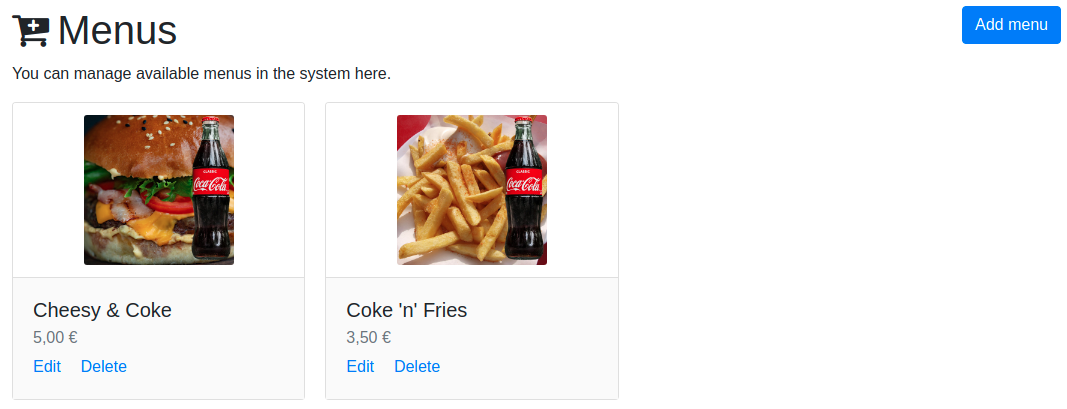
\includegraphics[width=0.8\textwidth]{images/ACP/menus.png}
    \caption{Die Menüsseite des Sokka-ACPs}
\end{figure}

Genau wie bei den Produkten, baut die Seite zum Hinzufügen von Menüs (erreichbar über den \glqq Add menu\grqq -Button) und dem Bearbeiten von Menüs (erreichbar über den \glqq Edit\grqq -Button in den einzelnen Menükarten) auf derselben React-Component auf, weshalb das Aussehen der beiden Seiten nahezu identisch ist.

Die verfügbaren und einstellbaren Eigenschaften für Menüs sind:

\begin{itemize}
    \item \textbf{Name}: Der Name des Menüs
    \item \textbf{Price}: Der Preis des Menüs in Euro
    \item \textbf{Category}: Die Kategorie des Menüs
    \item \textbf{Image}: Das Vorschaubild des Menüs
\end{itemize}

Ein Menü im Sokka-System besteht immer aus Produkten im Sokka-System. Jedem Produkt in einem Menü kann ein Titel zugewiesen werden, um die Rolle des Produkts im Menü anzuzeigen (beispielsweise \glqq Starter\grqq\space für Vorspeisen oder \glqq Main Dish\grqq\space für Hauptgänge)

\begin{figure}[ht]
    \centering
    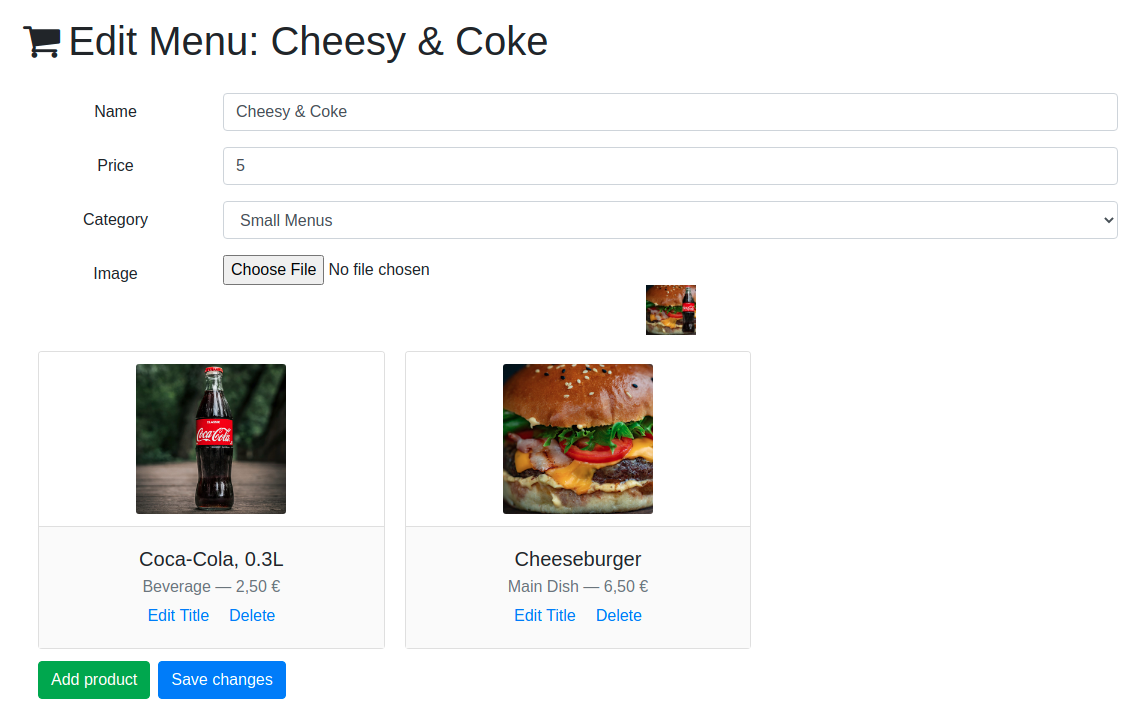
\includegraphics[width=0.6\textwidth]{images/ACP/menus_edit.png}
    \caption{Die Bearbeitungsseite von Menüs im Sokka-ACP}
\end{figure}

Produkte in einem Menü können über den \glqq Delete\grqq -Button entfernt werden oder deren Titel über den \glqq Edit Title\grqq -Button bearbeitet werden. Um ein neues Produkt in das Menü hinzuzufügen, kann der \glqq Add product\grqq -Button verwendet werden.

\begin{figure}[ht]
    \centering
    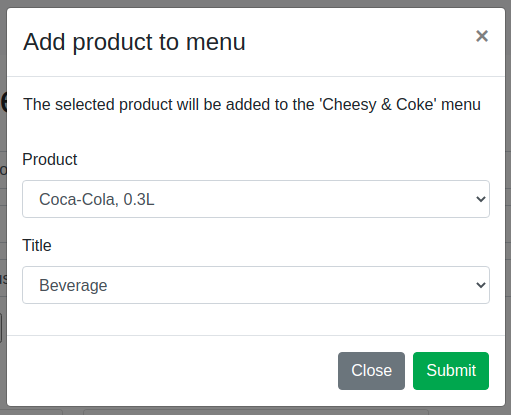
\includegraphics[width=0.6\textwidth]{images/ACP/menus_add_product.png}
    \caption{Dialog zum Hinzufügen neuer Produkte in einem Menü im Sokka-ACP}
\end{figure}